\documentclass[tikz]{standalone}
\tikzset{
  >=latex
}

\begin{document}
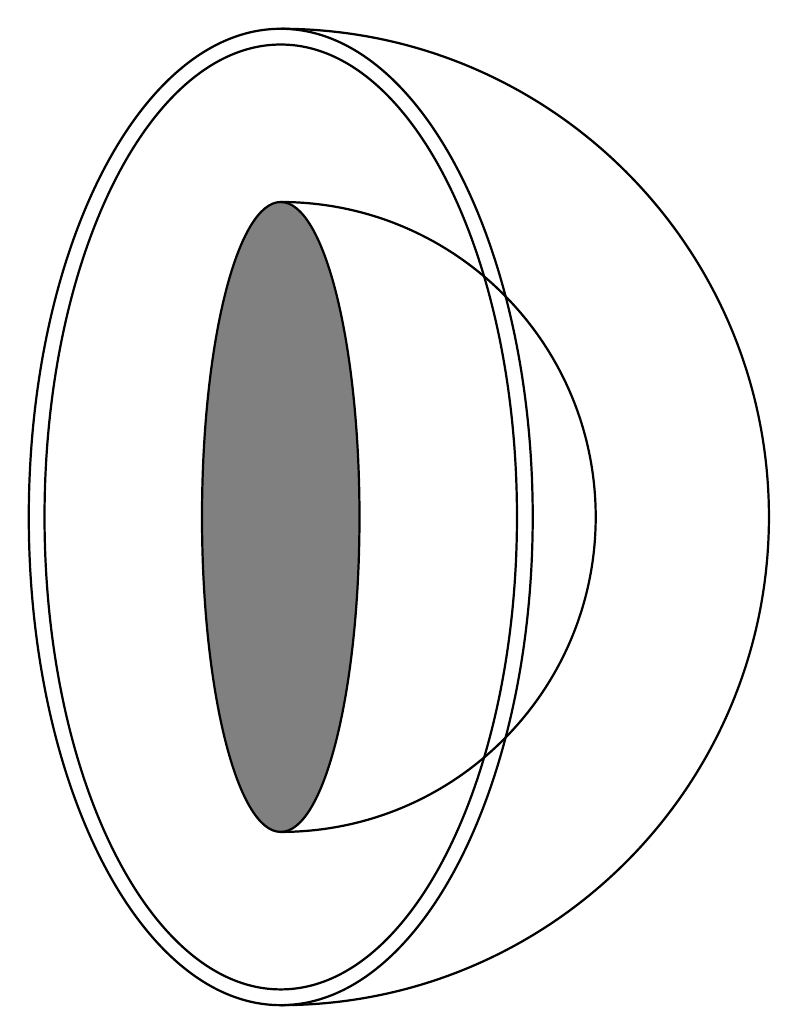
\begin{tikzpicture}
  \draw[thick,fill=gray](0,0) circle(1 and 4);
  \draw[thick] (0,-4) arc(-90:90:4);
  \draw[thick] (0,0) circle(3 and 6);
  \draw[thick] (0,0) circle(3.2 and 6.2);
  \draw[thick] (0,-6.2) arc(-90:90:6.2);
%  arc (0:180:2.5 and 1);
%  \draw(-2,8)--(-2,0);
%  \draw[dashed](-2,0) arc(180:0:2.5 and 1);
%  \draw(3,0)--(3,8) arc (0:180:2.5 and 1);
%
%  \fill[green, opacity=.1](-1,8)--(-1,0) arc(180:0:1.5 and .5) -- (2,8)
%  arc(0:180:1.5 and .5) -- (-1,8);
%  \draw[dashed,thick,red] (-1,8)--(-1,0) arc(180:0:1.5 and .5)
%  --(2,8) arc(0:180:1.5 and .5) -- (-1,8);
%
%  \fill[blue, opacity=.6](0,8)--(0,0) arc(180:0:.5 and .2) -- (1,8)
%  arc(0:180:.5 and .2) -- (0,8);
%  \draw (0,8)--(0,0);
%  \draw[dashed](0,0)arc(180:0:.5 and .2);
%  \draw(1,0)-- (1,8) arc(0:180:.5 and .2) -- (0,8);
%  
%  \draw[->](.5,0)--(.5,10) node[above]{$z$};
%  \draw[->,rotate around={-10:(.5,0)}](.5,0)--(4,0) node[right]{$x$};
%  \draw[->,rotate around={-155:(.5,0)}](.5,0)--(3.4,0) node[below]{$y$};
%  
%  \fill[blue, opacity=.7](0,8)--(0,0) arc(180:360:.5 and .2) -- (1,8)
%  arc(0:-180:.5 and .2) -- (0,8);
%  \draw (0,8)--(0,0) arc(180:360:.5 and .2);
%  \draw(1,0)-- (1,8) arc(0:-180:.5 and .2) -- (0,8);
%
%  \fill[green, opacity=.1](-1,8)--(-1,0) arc(180:360:1.5 and .5) -- (2,8)
%  arc(0:-180:1.5 and .5) -- (-1,8);
%  \draw[dashed,thick,red] (-1,8) arc(180:360:1.5 and .5);
%  \draw[dashed,thick,red] (-1,0) arc(180:360:1.5 and .5);
%  
%  \fill[pink,opacity=.5](-2,8)--(-2,0) arc(180:360:2.5 and 1)
%  --(3,8) arc (0:-180:2.5 and 1);
%  \draw(-2,8)--(-2,0) arc(180:360:2.5 and 1) --(3,8) arc (0:-180:2.5 and 1);
%
%  \draw[|<->|](3.3,8)--(3.3,0) node[midway,fill=white]{$L$};
%  \draw[->,rotate around={10:(.5,8)}](.5,8)--(.95,8) node[right]{$a$};
%  \draw[->,rotate around={-30:(.5,8)}](.5,8)--(2.15,8) node[below]{$b$};
\end{tikzpicture}
\end{document}
